% Created 2023-03-08 Wed 09:14
% Intended LaTeX compiler: pdflatex
\documentclass[presentation, t]{beamer}
\usepackage[utf8]{inputenc}
\usepackage[T1]{fontenc}
\usepackage{fontspec}
\usepackage{xcolor}
\usepackage{hyperref}
% features: (acronym underline par-sep beamer image .missing-koma)
\newcommand{\acr}[1]{\protect\textls*[110]{\scshape #1}}
\newcommand{\acrs}{\protect\scalebox{.91}[.84]{\hspace{0.15ex}s}}
\usepackage[normalem]{ulem}
\setlength{\parskip}{\baselineskip}
\setlength{\parindent}{0pt}

\usepackage{graphicx}
\usepackage{scrextend}
% end features

%% make document follow Emacs theme

\definecolor{obg}{HTML}{2E3440}
\definecolor{ofg}{HTML}{ECEFF4}

% heading colours
\definecolor{documentTitle}{HTML}{81A1C1}
\definecolor{documentInfo}{HTML}{81A1C1}
\definecolor{level1}{HTML}{81A1C1}
\definecolor{level2}{HTML}{B48EAD}
\definecolor{level3}{HTML}{5D80AE}
\definecolor{level4}{HTML}{a0b8d0}
\definecolor{level5}{HTML}{c6aac1}
\definecolor{level6}{HTML}{c0d0e0}
\definecolor{level7}{HTML}{d9c6d6}
\definecolor{level8}{HTML}{e5ecf2}

% textual elements

\definecolor{link}{HTML}{81A1C1}
\colorlet{url}{link}
\definecolor{cite}{HTML}{88C0D0}
\definecolor{itemlabel}{HTML}{81A1C1}
\definecolor{code}{HTML}{B48EAD}
\definecolor{verbatim}{HTML}{A3BE8C}

\DeclareTextFontCommand{\texttt}{\color{code}\ttfamily}

\let\oldverb\verb
\def\verb{\bgroup\color{verbatim}\oldverb}
\makeatletter
\let\verb@oldegroup\verb@egroup
\def\verb@egroup{\verb@oldegroup\egroup}
\makeatother

% beamer

\definecolor{builtin}{HTML}{81A1C1}
\definecolor{varname}{HTML}{D8DEE9}

\NewCommandCopy{\oldusetheme}{\usetheme}
\renewcommand*{\usetheme}[2][]{\oldusetheme[#1]{#2}
  \setbeamercolor{title separator}{fg=documentTitle}
  \setbeamercolor{progress bar}{fg=documentTitle}
  \setbeamercolor{progress bar in head/foot}{fg=documentTitle}
  \setbeamercolor{progress bar in section page}{fg=documentTitle}

  \setbeamercolor{normal text}{fg=ofg, bg=obg}
  \setbeamercolor{alerted text}{fg=varname}
  \setbeamercolor*{item}{fg=itemlabel}
  \setbeamercolor{block title}{fg=level3, bg=}
}

\usepackage{etoolbox}
\makeatletter
\patchcmd{\beamer@section}{%
  \edef\insertsectionhead{\noexpand\hyperlink{Navigation\the\c@page}{\unexpanded{#1}}}}{%
  \edef\insertsectionhead{\begingroup\noexpand\hypersetup{hidelinks}\noexpand\hyperlink{Navigation\the\c@page}{\unexpanded{#1}}\endgroup}}
\makeatother

% code blocks

\definecolor{codebackground}{HTML}{373E4C}
\colorlet{EFD}{ofg}
\definecolor{codeborder}{HTML}{404654}

%% end customisations

\usetheme[progressbar=foot]{metropolis}
\author{Ellis Kenyő}
\date{\today}
\title{State of Doom Emacs 2023}
\subtitle{\footnotesize Icon from @eccentric-j}
\titlegraphic{
\includegraphics[height=1.5cm]{doom.png}}
\usepackage{pgfpages}
\setbeameroption{show notes on second screen=right}
\setbeamertemplate{note page}{\insertnote\par}
\colorlet{greenyblue}{blue!70!green}
\colorlet{blueygreen}{blue!40!green}
\providecolor{link}{named}{greenyblue}
\providecolor{cite}{named}{blueygreen}
\hypersetup{
  pdfauthor={Ellis Kenyő},
  pdftitle={State of Doom Emacs 2023},
  pdfkeywords={},
  pdfsubject={},
  pdfcreator={Emacs 29.0.60 (Org mode 9.6.1)},
  pdflang={English},
  breaklinks=true,
  colorlinks=true,
  linkcolor=,
  urlcolor=link,
  citecolor=cite
}
\urlstyle{same}

% Setup for code blocks [1/2]

\usepackage{fvextra}

\fvset{%
  commandchars=\\\{\},
  highlightcolor=white!95!black!80!blue,
  breaklines=true,
  breaksymbol=\color{white!60!black}\tiny\ensuremath{\hookrightarrow}}

% Make line numbers smaller and grey.
\renewcommand\theFancyVerbLine{\footnotesize\color{black!40!white}\arabic{FancyVerbLine}}

\usepackage{xcolor}

% In case engrave-faces-latex-gen-preamble has not been run.
\providecolor{EfD}{HTML}{f7f7f7}
\providecolor{EFD}{HTML}{28292e}

% Define a Code environment to prettily wrap the fontified code.
\usepackage[breakable,xparse]{tcolorbox}
\DeclareTColorBox[]{Code}{o}%
{colback=EfD!98!EFD, colframe=EfD!95!EFD,
  fontupper=\footnotesize\setlength{\fboxsep}{0pt},
  colupper=EFD,
  IfNoValueTF={#1}%
  {boxsep=2pt, arc=2.5pt, outer arc=2.5pt,
    boxrule=0.5pt, left=2pt}%
  {boxsep=2.5pt, arc=0pt, outer arc=0pt,
    boxrule=0pt, leftrule=1.5pt, left=0.5pt},
  right=2pt, top=1pt, bottom=0.5pt,
  breakable}

% Support listings with captions
\usepackage{float}
\floatstyle{plain}
\newfloat{listing}{htbp}{lst}
\newcommand{\listingsname}{Listing}
\floatname{listing}{\listingsname}
\newcommand{\listoflistingsname}{List of Listings}
\providecommand{\listoflistings}{\listof{listing}{\listoflistingsname}}


% Setup for code blocks [2/2]: syntax highlighting colors

\newcommand\efstrut{\vrule height 2.1ex depth 0.8ex width 0pt}
\definecolor{EFD}{HTML}{ECEFF4}
\definecolor{EfD}{HTML}{2E3440}
\newcommand{\EFD}[1]{\textcolor{EFD}{#1}} % default
\newcommand{\EFvp}[1]{#1} % variable-pitch
\definecolor{EFh}{HTML}{4C566A}
\newcommand{\EFh}[1]{\textcolor{EFh}{#1}} % shadow
\definecolor{EFsc}{HTML}{A3BE8C}
\newcommand{\EFsc}[1]{\textcolor{EFsc}{#1}} % success
\definecolor{EFw}{HTML}{EBCB8B}
\newcommand{\EFw}[1]{\textcolor{EFw}{#1}} % warning
\definecolor{EFe}{HTML}{BF616A}
\newcommand{\EFe}[1]{\textcolor{EFe}{#1}} % error
\definecolor{EFl}{HTML}{81A1C1}
\newcommand{\EFl}[1]{\textcolor{EFl}{\textbf{#1}}} % link
\definecolor{EFlv}{HTML}{ee82ee}
\newcommand{\EFlv}[1]{\textcolor{EFlv}{\textbf{#1}}} % link-visited
\definecolor{EFhi}{HTML}{191C25}
\definecolor{Efhi}{HTML}{81A1C1}
\newcommand{\EFhi}[1]{\colorbox{Efhi}{\efstrut{}\textcolor{EFhi}{#1}}} % highlight
\definecolor{EFc}{HTML}{6f7787}
\newcommand{\EFc}[1]{\textcolor{EFc}{#1}} % font-lock-comment-face
\definecolor{EFcd}{HTML}{6f7787}
\newcommand{\EFcd}[1]{\textcolor{EFcd}{#1}} % font-lock-comment-delimiter-face
\definecolor{EFs}{HTML}{A3BE8C}
\newcommand{\EFs}[1]{\textcolor{EFs}{#1}} % font-lock-string-face
\definecolor{EFd}{HTML}{78808f}
\newcommand{\EFd}[1]{\textcolor{EFd}{#1}} % font-lock-doc-face
\definecolor{EFm}{HTML}{81A1C1}
\newcommand{\EFm}[1]{\textcolor{EFm}{#1}} % font-lock-doc-markup-face
\definecolor{EFk}{HTML}{81A1C1}
\newcommand{\EFk}[1]{\textcolor{EFk}{#1}} % font-lock-keyword-face
\definecolor{EFb}{HTML}{81A1C1}
\newcommand{\EFb}[1]{\textcolor{EFb}{#1}} % font-lock-builtin-face
\definecolor{EFf}{HTML}{88C0D0}
\newcommand{\EFf}[1]{\textcolor{EFf}{#1}} % font-lock-function-name-face
\definecolor{EFv}{HTML}{D8DEE9}
\newcommand{\EFv}[1]{\textcolor{EFv}{#1}} % font-lock-variable-name-face
\definecolor{EFt}{HTML}{8FBCBB}
\newcommand{\EFt}[1]{\textcolor{EFt}{#1}} % font-lock-type-face
\definecolor{EFo}{HTML}{81A1C1}
\newcommand{\EFo}[1]{\textcolor{EFo}{#1}} % font-lock-constant-face
\definecolor{EFwr}{HTML}{EBCB8B}
\newcommand{\EFwr}[1]{\textcolor{EFwr}{#1}} % font-lock-warning-face
\definecolor{EFnc}{HTML}{81A1C1}
\newcommand{\EFnc}[1]{\textcolor{EFnc}{\textbf{#1}}} % font-lock-negation-char-face
\definecolor{EFpp}{HTML}{81A1C1}
\newcommand{\EFpp}[1]{\textcolor{EFpp}{\textbf{#1}}} % font-lock-preprocessor-face
\definecolor{EFrc}{HTML}{81A1C1}
\newcommand{\EFrc}[1]{\textcolor{EFrc}{\textbf{#1}}} % font-lock-regexp-grouping-construct
\definecolor{EFrb}{HTML}{81A1C1}
\newcommand{\EFrb}[1]{\textcolor{EFrb}{\textbf{#1}}} % font-lock-regexp-grouping-backslash
\definecolor{Efob}{HTML}{373E4C}
\newcommand{\EFob}[1]{\colorbox{Efob}{\efstrut{}#1}} % org-block
\definecolor{EFobb}{HTML}{6f7787}
\definecolor{Efobb}{HTML}{373E4C}
\newcommand{\EFobb}[1]{\colorbox{Efobb}{\efstrut{}\textcolor{EFobb}{#1}}} % org-block-begin-line
\definecolor{EFobe}{HTML}{6f7787}
\definecolor{Efobe}{HTML}{373E4C}
\newcommand{\EFobe}[1]{\colorbox{Efobe}{\efstrut{}\textcolor{EFobe}{#1}}} % org-block-end-line
\definecolor{EFOa}{HTML}{81A1C1}
\newcommand{\EFOa}[1]{\textcolor{EFOa}{\textbf{#1}}} % outline-1
\definecolor{EFOb}{HTML}{B48EAD}
\newcommand{\EFOb}[1]{\textcolor{EFOb}{\textbf{#1}}} % outline-2
\definecolor{EFOc}{HTML}{5D80AE}
\newcommand{\EFOc}[1]{\textcolor{EFOc}{\textbf{#1}}} % outline-3
\definecolor{EFOd}{HTML}{a0b8d0}
\newcommand{\EFOd}[1]{\textcolor{EFOd}{\textbf{#1}}} % outline-4
\definecolor{EFOe}{HTML}{c6aac1}
\newcommand{\EFOe}[1]{\textcolor{EFOe}{\textbf{#1}}} % outline-5
\definecolor{EFOf}{HTML}{c0d0e0}
\newcommand{\EFOf}[1]{\textcolor{EFOf}{\textbf{#1}}} % outline-6
\definecolor{EFOg}{HTML}{d9c6d6}
\newcommand{\EFOg}[1]{\textcolor{EFOg}{\textbf{#1}}} % outline-7
\definecolor{EFOh}{HTML}{e5ecf2}
\newcommand{\EFOh}[1]{\textcolor{EFOh}{\textbf{#1}}} % outline-8
\definecolor{EFhn}{HTML}{B48EAD}
\newcommand{\EFhn}[1]{\textcolor{EFhn}{\textbf{#1}}} % highlight-numbers-number
\definecolor{EFhq}{HTML}{81A1C1}
\newcommand{\EFhq}[1]{\textcolor{EFhq}{#1}} % highlight-quoted-quote
\definecolor{EFhs}{HTML}{8FBCBB}
\newcommand{\EFhs}[1]{\textcolor{EFhs}{#1}} % highlight-quoted-symbol
\definecolor{EFrda}{HTML}{81A1C1}
\newcommand{\EFrda}[1]{\textcolor{EFrda}{#1}} % rainbow-delimiters-depth-1-face
\definecolor{EFrdb}{HTML}{B48EAD}
\newcommand{\EFrdb}[1]{\textcolor{EFrdb}{#1}} % rainbow-delimiters-depth-2-face
\definecolor{EFrdc}{HTML}{A3BE8C}
\newcommand{\EFrdc}[1]{\textcolor{EFrdc}{#1}} % rainbow-delimiters-depth-3-face
\definecolor{EFrdd}{HTML}{5D80AE}
\newcommand{\EFrdd}[1]{\textcolor{EFrdd}{#1}} % rainbow-delimiters-depth-4-face
\definecolor{EFrde}{HTML}{8FBCBB}
\newcommand{\EFrde}[1]{\textcolor{EFrde}{#1}} % rainbow-delimiters-depth-5-face
\definecolor{EFrdf}{HTML}{81A1C1}
\newcommand{\EFrdf}[1]{\textcolor{EFrdf}{#1}} % rainbow-delimiters-depth-6-face
\definecolor{EFrdg}{HTML}{B48EAD}
\newcommand{\EFrdg}[1]{\textcolor{EFrdg}{#1}} % rainbow-delimiters-depth-7-face
\definecolor{EFrdh}{HTML}{A3BE8C}
\newcommand{\EFrdh}[1]{\textcolor{EFrdh}{#1}} % rainbow-delimiters-depth-8-face
\definecolor{EFrdi}{HTML}{5D80AE}
\newcommand{\EFrdi}[1]{\textcolor{EFrdi}{#1}} % rainbow-delimiters-depth-9-face
\definecolor{EFany}{HTML}{EBCB8B}
\definecolor{Efany}{HTML}{EBCB8B}
\newcommand{\EFany}[1]{\colorbox{Efany}{\efstrut{}\textcolor{EFany}{#1}}} % ansi-color-yellow
\definecolor{EFanr}{HTML}{BF616A}
\definecolor{Efanr}{HTML}{BF616A}
\newcommand{\EFanr}[1]{\colorbox{Efanr}{\efstrut{}\textcolor{EFanr}{#1}}} % ansi-color-red
\definecolor{EFanb}{HTML}{2E3440}
\newcommand{\EFanb}[1]{\textcolor{EFanb}{#1}} % ansi-color-black
\definecolor{EFang}{HTML}{A3BE8C}
\definecolor{Efang}{HTML}{A3BE8C}
\newcommand{\EFang}[1]{\colorbox{Efang}{\efstrut{}\textcolor{EFang}{#1}}} % ansi-color-green
\definecolor{EFanB}{HTML}{81A1C1}
\definecolor{EfanB}{HTML}{81A1C1}
\newcommand{\EFanB}[1]{\colorbox{EfanB}{\efstrut{}\textcolor{EFanB}{#1}}} % ansi-color-blue
\definecolor{EFanc}{HTML}{88C0D0}
\definecolor{Efanc}{HTML}{88C0D0}
\newcommand{\EFanc}[1]{\colorbox{Efanc}{\efstrut{}\textcolor{EFanc}{#1}}} % ansi-color-cyan
\definecolor{Efanw}{HTML}{ECEFF4}
\newcommand{\EFanw}[1]{\colorbox{Efanw}{\efstrut{}#1}} % ansi-color-white
\definecolor{EFanm}{HTML}{B48EAD}
\definecolor{Efanm}{HTML}{B48EAD}
\newcommand{\EFanm}[1]{\colorbox{Efanm}{\efstrut{}\textcolor{EFanm}{#1}}} % ansi-color-magenta
\definecolor{EFANy}{HTML}{edd29c}
\definecolor{EfANy}{HTML}{edd29c}
\newcommand{\EFANy}[1]{\colorbox{EfANy}{\efstrut{}\textcolor{EFANy}{#1}}} % ansi-color-bright-yellow
\definecolor{EFANr}{HTML}{c87880}
\definecolor{EfANr}{HTML}{c87880}
\newcommand{\EFANr}[1]{\colorbox{EfANr}{\efstrut{}\textcolor{EFANr}{#1}}} % ansi-color-bright-red
\definecolor{EFANb}{HTML}{191C25}
\definecolor{EfANb}{HTML}{2C333F}
\newcommand{\EFANb}[1]{\colorbox{EfANb}{\efstrut{}\textcolor{EFANb}{#1}}} % ansi-color-bright-black
\definecolor{EFANg}{HTML}{b0c79d}
\definecolor{EfANg}{HTML}{b0c79d}
\newcommand{\EFANg}[1]{\colorbox{EfANg}{\efstrut{}\textcolor{EFANg}{#1}}} % ansi-color-bright-green
\definecolor{EFANB}{HTML}{93afca}
\definecolor{EfANB}{HTML}{93afca}
\newcommand{\EFANB}[1]{\colorbox{EfANB}{\efstrut{}\textcolor{EFANB}{#1}}} % ansi-color-bright-blue
\definecolor{EFANc}{HTML}{99c9d7}
\definecolor{EfANc}{HTML}{99c9d7}
\newcommand{\EFANc}[1]{\colorbox{EfANc}{\efstrut{}\textcolor{EFANc}{#1}}} % ansi-color-bright-cyan
\definecolor{EFANw}{HTML}{F0F4FC}
\definecolor{EfANw}{HTML}{F0F4FC}
\newcommand{\EFANw}[1]{\colorbox{EfANw}{\efstrut{}\textcolor{EFANw}{#1}}} % ansi-color-bright-white
\definecolor{EFANm}{HTML}{bf9eb9}
\definecolor{EfANm}{HTML}{bf9eb9}
\newcommand{\EFANm}[1]{\colorbox{EfANm}{\efstrut{}\textcolor{EFANm}{#1}}} % ansi-color-bright-magenta
\begin{document}

\maketitle

\note{
\tiny

Welcome everyone to my ``State of Doom'' talk. There's been a decent amount of
discussion recently in Slack around Doom so I thought I'd do my best to fill
everyone in on exactly what Doom is, what's happened recently and some exciting
things coming soon.

There will also be a very short walkthrough of installing and running the ootb
setup, assuming the demo Gods allow it to be.}

\section{What is Doom Emacs?}
\label{sec:org59372d2}
\begin{frame}[label={sec:org6fe2c85}]{What is Doom Emacs?}
\begin{itemize}
\item A modular config framework
\item Similar to Spacemacs, Prelude, Centaur Emacs
\item Batteries-included Emacs
\item Sensible but (somewhat) opinionated defaults
\item Package management \emph{outside} Emacs and \emph{declarative}
\item Optimized around startup time
\end{itemize}

\note{
\tiny

Well, put simply; Doom is a modular configuration framework built for Emacs.
Similar in nature to Spacemacs, it aims to provide a more batteries-included
experience for Emacs by providing what we've deemed as sensible but (somewhat,
less so recently) opinionated defaults.

However, unlike other frameworks; Doom aims to keep the package management
outside of Emacs (you don't want everything to download/update when you start
Emacs) and also aims to be as declarative as possible (more on the future of
this later) meaning that you can easily pin packages to specific versions and
they'll only pull new updates when you update the pin.}
\end{frame}

\begin{frame}[label={sec:orgd96070b}]{A Brief History of Doom}
\begin{itemize}
\item Created by Henrik Lissner (@hlissner)
\item Started as his private config
\item Initially structured like Prelude, shortly made to be modular
\end{itemize}

\note{
\tiny

So where did this all come from? Doom wasn't created with a starter kit/config
framework in mind, it just began as Henrik Lissner (the initial and current
maintainer) decided to try and build his own config as an attempt to learn Emacs
Lisp. Starting out a bit like Prelude, it was later migrated to be based around
pluggable modules and incorporated things like Spacemacs' leader key from
migrating users.}
\end{frame}

\begin{frame}[label={sec:org6f69023},fragile]{What is a module?}
 \begin{itemize}
\item Collection of packages with glue
\item Grouped by a class and can include optional flags
\item Looks like \texttt{:editor lsp +eglot}
\end{itemize}

\note{
\tiny

Okay we've heard this term ``modular'' used quite a few times, but what exactly is
it? Simply put, it's a collection of packages with some extra code to integrate
them together. For example, the Clojure module currently pulls in \texttt{clojure-mode},
\texttt{paredit}, \texttt{clj-refactor} and \texttt{flycheck-clj-kondo} (when the syntax check module is
enabled) and most of the configuration is moving the keybindings to be focused
around the leader key (eg \texttt{SPC m '} for \texttt{cider-jack-in}'), integrating with Doom's
popup system and some LSP config (when the LSP module is enabled).

Each module is grouped by a number of keywords and can include optional flags
denoted by a plus. The example we have there is the LSP module with eglot
support optionally enabled.}
\end{frame}

\begin{frame}[label={sec:org728ea40},fragile]{\texttt{doom} CLI}
 \tiny
\begin{Code}
\begin{Verbatim}
\color{EFD}doom sync
\end{Verbatim}
\end{Code}

\begin{verbatim}
> Tangling your literate config...
  ✓ Done tangling 5 file(s)!
> Synchronizing "default" profile...
  > Regenerating envvars file
    ✓ Generated ~/.config/emacs/.local/env
  > Installing packages...
    - No packages need to be installed
  > (Re)building packages...
    - No packages need rebuilding
  > Purging orphaned packages (for the emperor)...
    - Skipping builds
    - Skipping elpa packages
    - Skipping repos
    - Skipping regrafting
    - Skipping native bytecode
  > (Re)building profile in /home/elken/.config/emacs/.local/etc/@/...
    > Deleting old init files...
    > Generating 4 init files...
    > Byte-compiling ~/.config/emacs/.local/etc/@init.29.el...
    ✓ Built init.29.elc
  - Restart Emacs or use 'M-x doom/reload' for changes to take effect
\end{verbatim}

\note{
\tiny

I mentioned before the Doom offloads a lot to a CLI tool, but what exactly for?
The primary purpose is to perform an operation called \texttt{sync} which will perform
any defined package management options (and if you're using a literate org-based
config, that will get tangled first) and also run through a number of internal
steps such as building, clearing orphaned packages and something we'll touch
shortly at the bottom for rebuilding the profile.

You can also do \texttt{doom sync -u} when you need to update all the package versions
you have, or when you update the pin on a package or packages. \texttt{doom upgrade} to
pull in the latest changes from Doom itself and also perform a \texttt{doom sync -u}.}
\end{frame}


\begin{frame}[label={sec:org9467204},fragile]{\texttt{doom} CLI}
 \begin{center}
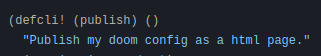
\includegraphics[width=.9\linewidth]{cli_publish.png}
\end{center}

\begin{Code}
\begin{Verbatim}
\color{EFD}doom help | rg \EFs{"publish"}
\end{Verbatim}
\end{Code}

\begin{verbatim}
publish    Publish my doom config as a html page.
\end{verbatim}

\note{
\tiny

And by far the \emph{coolest} feature available is you can very easily extend this to
provide your own CLI tools. This screenshot is just the macro from my Doom
config to publish my config as HTML, borrowing a couple of other tecosaur
packages to produce nicer output. The script is called \texttt{publish}, and the
docstring is shown in the help menu. I can call this with \texttt{doom publish} so long
as that cli.el file is present.}
\end{frame}

\section{Demo}
\label{sec:org50a1971}
\section{What's changed recently?}
\label{sec:orgec77da3}
\begin{frame}[label={sec:orga20f564},fragile]{Profiles}
 \begin{itemize}
\item Largest recent change
\item Still more changes to come
\item Generational, similar to Nix
\end{itemize}
\note{
\tiny

So what's new lately? The largest recent change has been the introduction of a
profile system. If you remember from the output of \texttt{doom sync}, at the
bottom there was mention of profiles being updated.

Powering something that will be talked about shortly (transactional package
management), a profile system was introduced to act as an improved version of
Chemacs (a tool for running multiple Emacs configs side-by-side).

Outside of the main profile which pertains to your config, you can place extras
inside your private Doom config directory under a \texttt{profiles} folder.

The profiles system has a lot more changes coming soon, such as being able to
generate profiles for use in the sandbox and the upcoming transactional package
management changes.}
\end{frame}

\begin{frame}[label={sec:org98e4b67},fragile]{New modules}
 \begin{itemize}
\item \texttt{:lang graphql}
\item \texttt{:tools tree-sitter}
\item More coming soon
\end{itemize}
\note{
\tiny

A couple of new modules have been added, a simple graphql module added by me
which provides a sane graphql experience and has improved support for a
\texttt{.graphqlconfig} file. The LSP server is a bit buggy, thanks to the complexity of
node packaging, but for the most part completion and running queries should work
as expected. It also includes org-babel support for running graphql queries.

As well as that, predating Emacs 29 getting tree-sitter support (and as such
needing a refactor to better integrate) support was added for tree-sitter and
any modules that had grammars defined. This also included extra text objects for
evil users, with proposed support for integrating tree-edit.}
\end{frame}

\begin{frame}[label={sec:orgb3894d6}]{Docs progress}
\begin{itemize}
\item \url{https://docs.doomemacs.org/latest/}
\item Viewing in Emacs is the best way
\end{itemize}
\note{
\tiny

Every developer's favourite thing; writing documentation. For a while, most of the knowledge not part of module READMEs was in Henrik's head making contribution in some cases difficult. This has been changing as more and more module maintainers have been introduced and the project shifts to being much more modular.

As such, a push to greatly improve the quality of the documentation is on-going; as well as improvements to viewing the docs inside Emacs, including things like conditionally highlighting modules and packages based on whether or not you've installed them.}
\end{frame}

\section{What's coming next?}
\label{sec:orgab8906d}
\begin{frame}[label={sec:orgbfeea96},fragile]{Doom v3 (this time, without The Rock)}
 \vspace*{-30pt}
\footnotesize
\begin{columns}
\begin{column}{0.8\columnwidth}
\begin{block}{}
\begin{itemize}
\item Splitting up into core, modules \& community modules
\item Transactional package management
\item Generalizing the Doom CLI
\item CI/CD for automating package bumping and tests
\item On-the-fly profile generation
\item On-the-fly module activation
\item Recursive modules
\item Managing external module libraries like you can packages
\item An installation wizard for \texttt{doom install}
\item Upcoming modules
\begin{itemize}
\item \texttt{:completion corfu}
\item \texttt{:editor format} refactor
\item \texttt{:config tutorial}
\end{itemize}
\end{itemize}
\end{block}
\end{column}

\begin{column}{0.3\columnwidth}
\begin{block}{}
\begin{center}

\includegraphics[width=\textwidth]{the_rock.png}
\end{center}
\end{block}
\end{column}
\end{columns}


\note{
\tiny

First up, splitting up the core pieces of doom. People have been asking for some time now about having access to a few bits of Doom without having to include everything else, so everything will be split into core, the core modules and community modules.

Next we have transactional package management. Similar to Nix, each ``change'' to the packages in a profile will constitute a new generation that can be rolled back to at any point and managed similarly to any other profile.

Then we have some generalizing of the Doom CLI code to become a general-purpose tool for elisp development, providing things like linting, tests, etc. Similar to cask, eask or eldev.

Improved CI is self-explanatory, automate some of the more annoying tasks like bumping packages and add tests; all managed via a github action.

Profile generation on-the-fly relates to the sandbox, and being able to create a slightly less transient sandbox that you can even use Nix to deploy to specific Emacs versions.

Only-the-fly module activation is the simple act of the first time a file is opened that there is a module for, prompt the user asking if they wish to install said module.

Recursive modules solves a problem we hit recently where both the F\# and C\# modules have a shared dependency, but also different sets of dependencies that you won't need for either language, so the simplest way to solve this was to introduce a kind of ``meta module'' under \texttt{dotnet} but also allow you to selectively install just the languages you care about, without having to manage multiple sets of pins.

Then we have the ability to manage external modules as you do with packages, being able to pin, version, profile, etc.

Also on the cards is a simplified installation wizard during installation to let users tailor their installation easier.

And finally we have a few new modules working through, adding in corfu as a completion frontend with the view to replace company, a large refactor of all the \texttt{:editor format} components by me to use apheleia instead, and a module for creating interactive tutorials in Emacs by tecosaur.}
\end{frame}


\begin{frame}[label={sec:orgdd4ed38}]{Where you can find us}
\begin{itemize}
\item \url{https://doomemacs.org/discord}
\item \url{https://discourse.doomemacs.org/}
\item \url{https://github.com/doomemacs}
\end{itemize}

\note{
\tiny

That's just a taster though, if you're more interested there's a couple of links here to find us. There's been talk of moving away from Discord to Matrix, but until that materializes that's the best place to reach us in terms of following the project (outside of Github obviously). The recent addition of the Discourse server to better facilitate Q\&A has also gone well, and is much more convenient for posting questions and getting answers to them, but the forum channels on the Discord also exist.}
\end{frame}

\section{Any Questions?}
\label{sec:org270e4ee}
\end{document}
